\def\theTopic{Reading 7}
 %% was reading 9 in Spring 2016

\section{ The Sampling Distribution}


 Statistical inference is based on simple ideas of random treatment
 assignment, random selection, and random sampling.   {\bf RANDOM} 
 means that the outcome we will get cannot be known, but the
 distribution of possible outcomes can be known. 


\subsection{ Sampling Distribution for $\phat$}

 Consider selecting a random sample of 100 people with season passes
 to a local ski run and asking if they snow board more than they ski.
 Our sample will produce a sample  proportion -- a number which we
 cannot know ahead of time.  We will only select 
 one sample, and will only get to see one sample proportion, but we
 can think about the process of random selection and consider all the
 sample proportions we might have obtained.  This is a powerful way to
 think abstractly about the random selection process:
 \begin{itemize}
 \item We observe one sample.
 \item What else might we have observed?
 \end{itemize}
  The {\bf sampling distribution} is a description of all possible
  outcomes and the probabilities of obtaining each outcome.  If, for
  example, actually 48.7\%  of season pass holders board, then we
  could use a spinner to simulate the sampling distribution and would
  get a picture like this:

  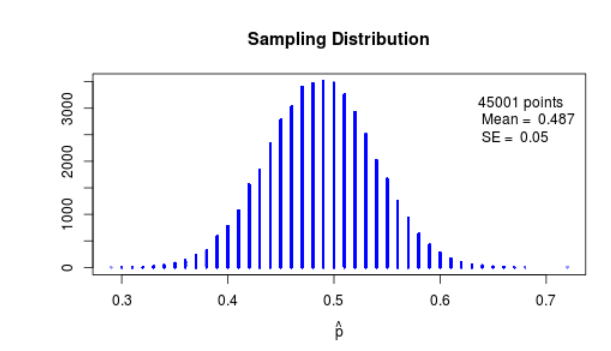
\includegraphics[width=.5\linewidth]{../plots/SampDistnofPhat-100.png}

It is centered at the true value, 0.487 as the proportion of boarders,
and has spread indicated by $SE(\phat) = 0.05$. 
%  If we decide to
% increase the sample size to 1000, the center will stay the same, but
% the spread will get smaller.
It would be very useful to know the sampling distribution so that we
could find the center part of the distribution for a confidence
interval.  

Sampling distribution for $\phat$ depends on two things: the true
parameter $p$ (unknown), and the sample size, $n$. As sample size
increases, spread gets smaller. \vspace{1in}

\subsection{ Sampling Distribution for $\xbar$}

 Now suppose we are interested in the average age of season pass
 holders in a sample of size 100. The sampling distribution  for the
 sample mean age, $\xbar$, 
 again depends on the  unknown parameter which is now $\mu$, the true
 mean age in the population,  and sample size, $n$,
 but it also depends on the spread in the original distribution,
 $\sigma$.  
 The left hand pair of plots below is for individual season pass
 holders created (not real data) under two different assumed values
 for spread, either $\sigma = 5.5$ or $\sigma = 8$.

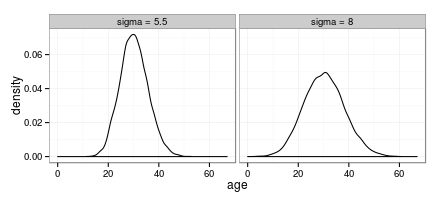
\includegraphics[width =.48\linewidth]{plots/twoSampDensities4x.png}
\hfill
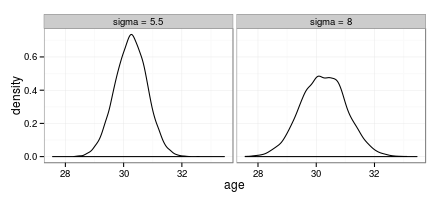
\includegraphics[width =.48\linewidth]{plots/twoSampDensities4xbar.png}\\

 The right hand pair of plots  shows the distributions of {\bf MEAN ages of 100
   season pass holders.} 

 A common confusion is to think that means will have the same
 distribution as the individuals. The distributions will have the
 same centers, but when we average to get means, we pull in the
 extreme points.  The distributions of individual ages (left) extend
 further to cover younger and older ages, but when averaged over 100
 people (right) those extreme values which rarely occur get pulled
 toward the center by the rest of the sample and we rarely see a
 sample {\bf average} as low as 28 or as high as 33.

 The distributions shown have the same means $\mu$, and the same $n =
 100$. The different values for $\sigma$ change the sampling
 distributions for $\xbar$, the sample mean.  



 

{\bf Important Points}
\begin{itemize}
\item What does it mean to say that an outcome is ``random''?\vfill
\item Why does a plot of a sampling distribution show many points, not
  just one? After all, there is just one sample, right?\vfill
\item Sampling distributions of $\phat$ and of $\xbar$ both depend on:
  \vfill
\item Additionally, the sampling distribution for $\xbar$ depends
  on:\vfill
\item Why is the sampling distribution for $\xbar$ less spread out
  than the distribution of the original data?
\end{itemize}


%% R code
% require(ggplot2)
% sample1 <- apply(matrix(rpois(1000000,30.25), nrow=100),2,mean)
% sample2 <- apply(matrix(rpois(1000000,60.25)-30, nrow=100),2,mean)
%  sampMeanFrame <- data.frame(age = c(sample1, sample2), sample = gl(2,
%  10000, labels = c("sigma = 5.5", "sigma = 8")))
%  qplot( x = age,  facets =  ~ sample, data = sampMeanFrame, geom = "density") + theme_bw()
% dev.copy(png,file = "plots/twoSampDensities4xbar.png",height = 200,
% width = 440);dev.off()

%  sample1 <- rpois(10000,30.25)
%  sample2 <- rpois(10000,64.25)-34
%   sampXFrame <- data.frame(age = c(sample1, sample2), sample = gl(2,
%   10000, labels = c("sigma = 5.5", "sigma = 8")))
%   qplot( x = age,  facets =  ~ sample, data = sampXFrame, geom =
%   "density", adjust = 1)  + theme_bw()
%  dev.copy(png,file = "plots/twoSampDensities4x.png",height = 200, width = 440);dev.off()